\section{Đề ôn thi giữa kỳ 2 toán 11}
\subsection{Phần trắc nghiệm}
Câu trắc nghiệm nhiều phương án lựa chọn. Học sinh trả lời từ
câu 1 đến câu 12. Mỗi câu hỏi học sinh \textit{chỉ chọn một} phương án.

\Opensolutionfile{ans}[Ans/Dapan]
 
\hienthiloigiaiex
%%%=============EX_1=============%%%
\begin{ex}%[1D6H1-2]
	Biểu thức $P=\sqrt[3]{x\sqrt[5]{x^2\sqrt{x}}}=x^{\alpha }$ (với $x>0$), giá trị của $\alpha $ là
	\choice
		{\True $\dfrac{1}{2}$}
		{$\dfrac{5}{2}$}
		{$\dfrac{9}{2}$}
		{$\dfrac{3}{2}$}
	\loigiai{
		$P=\sqrt[3]{x\sqrt[5]{x^2\sqrt{x}}}=\sqrt[3]{x\sqrt[5]{{x^{2}}\cdot{x^{\tfrac{1}{2}}}}}=\sqrt[3]{x\cdot{{\left( {x^{\tfrac{5}{2}}} \right)}^{\tfrac{1}{5}}}}={{\left( {x^{\tfrac{3}{2}}} \right)}^{\tfrac{1}{3}}}={x^{\tfrac{1}{2}}}\Rightarrow \alpha =\dfrac{1}{2}.$
		}
\end{ex}
%%%=============EX_2=============%%%
\begin{ex}%[1D6H1-4]
	Cho $(\sqrt{2}-1)^m<(\sqrt{2}-1)^n$. Khi đó
	\choice
		{$m=n$}
		{$m<n$}
		{\True $m>n$}
		{$m\ne n$}
	\loigiai{
		Do $0<\sqrt{2}-1<1$ nên $(\sqrt{2}-1)^m<(\sqrt{2}-1)^n\Leftrightarrow m>n$.
		}
\end{ex}

\begin{ex}%[1D6N2-2]
	Cho $a$, $b$, $c>0$, $a\ne 1$ và số $\alpha \in \mathbb{R}$, mệnh đề nào dưới đây \textbf{sai}?	
	\choice
		{${\log }_a{a^c}=c$}
		{${\log }_a a=1$}
		{${\log }_a{b^{\alpha }}=\alpha {\log }_a b$}
		{\True ${\log }_a\left| b-c \right|={\log }_a b-{\log }_a c$}
	\loigiai{
		Theo tính chất của logarit, mệnh đề sai là ${\log }_a\left| b-c \right|={\log }_a b-{\log }_a c$.
		}
\end{ex}
  
\begin{ex}%[1D6H2-2]
	Với $a$, $b$ là hai số dương tùy ý, $\log \left(ab^2\right)$ bằng
	\choice
		{$2\left( \log a+\log b \right)$}
		{$\log a+\dfrac{1}{2}\log b$}
		{$2\log a+\log b$}
		{\True $\log a+2\log b$}
	\loigiai{
		Có $\log \left(ab^2\right)=\log a+\log{b^2}=\log a+2\log b$.
		}
\end{ex}
  
\begin{ex}%[1D6N3-2]
	Tập xác định của hàm số $y=\log _3(x-4)$ là 
	\choice
		{$(5;+\infty)$}
		{$(-\infty ;+\infty)$}
		{\True $(4;+\infty)$}
		{$(-\infty ;4)$}
	\loigiai{
		Điều kiện ${x-4>0\Leftrightarrow x>4}$.
		Tập xác định $\mathscr{D}=(4;+\infty)$.
		}
\end{ex}
  
\begin{ex}%[1D6N3-3]
	Hàm số nào dưới đây đồng biến trên khoảng $(0;+\infty)$?
	\choice
		{\True $y={{\log }_{\sqrt{3}}}x$}
		{$y={\log }_{\dfrac{\pi }{6}}x$}
		{$y={\log }_{\dfrac{e}{3}}x$}
		{$y={\log }_{\dfrac{1}{4}}x$}
	\loigiai{
		Hàm số $y={\log }_a x$ đồng biến trên khoảng $(0;+\infty )\Leftrightarrow a>1$.
		}
\end{ex}
  
\begin{ex}%[1D6N4-2]
	Nghiệm của phương trình $\log _2(x-1)=3$ là
	\choice
		{$x=10$}
		{$x=8$}
		{\True $x=9$}
		{$x=7$}
	\loigiai{
		Ta có $\log _2(x-1)=3 \Leftrightarrow\left\{\begin{array}{l}x-1>0 \\ x-1=2^3\end{array} \Leftrightarrow\left\{\begin{array}{l}x>1 \\ x=9\end{array} \Leftrightarrow x=9\right.\right.$.
		}
\end{ex}
  
\begin{ex}%[1D6H4-5]
	Tập nghiệm của bất phương trình $3^{x^2-13}<27$ là
	\choice
		{$(4;+\infty)$}
		{\True $(-4;4)$}
		{$(-\infty;4)$}
		{$(0;4)$}
	\loigiai{
		Ta có $3^{x^2-13}<27\Leftrightarrow 3^{x^2-13}<3^3\Leftrightarrow x^2-13<3\Leftrightarrow x^2<16\Leftrightarrow \left| x \right|<4\Leftrightarrow -4<x<4$.\\
		Vậy tập nghiệm của bất phương trình đã cho là $S=(-4;4)$.
		}
\end{ex}
  
\begin{ex}%[1H8V1-2]
	Trong hình hộp $ABCD.A'B'C'D'$ có tất cả các cạnh đều bằng nhau. Trong các mệnh đề sau, mệnh đề nào sai?
	\choice
		{\True $BB'\perp BD$}
		{$A'C'\perp BD$}
		{$A'B\perp DC'$}
		{$BC'\perp A'D$}
	\loigiai{
		\immini{Vì hình hộp $ABCD.A'B'C'D'$ có tất cả các cạnh đều bằng nhau nên các tứ giác $ABCD$, $A'B'BA$, $B'C'CB$ đều là hình thoi nên ta có\\
		$AC\perp BD$ mà $AC\parallel A'C'\Rightarrow A'C'\perp BD$ (đúng).\\
		$A'B\perp AB'$ mà $AB'\parallel DC'\Rightarrow A'B\perp DC'$ (đúng).\\
		$BC'\perp B'C$ mà $B'C\parallel A'D\Rightarrow BC'\perp A'D$ (đúng).}
		{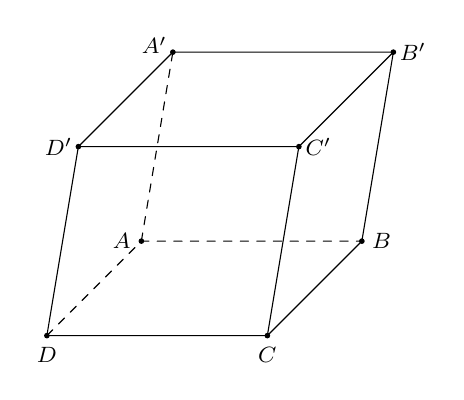
\begin{tikzpicture}[scale=0.8, font=\footnotesize, line join=round, line cap=round, >=stealth]
			\path
			(0,0) coordinate (D) 
			(3.5,0) coordinate (C) 
			(1.5,1.5) coordinate (A) 
			(A)+(3.5,0) coordinate (B);
			\foreach \x in {A,B,C,D}
			\path (\x)+(0.5,3) coordinate(\x');	
			\draw[dashed] (D)--(A)--(B) (A)--(A');
			\draw(D')--(C')--(B')--(A')--(D')--(D)--(C)--(B)--(B') (C)--(C');
			\foreach \p/\g in {D/-90,C/-90,B/0,A/180,D'/180,C'/0,B'/0,A'/160}\draw[fill=black] (\p) circle (1pt)node[shift={(\g:.25)}]{$\p$};
			\end{tikzpicture}}
		}
\end{ex}
  
\begin{ex}%[1H8H1-3]
	\immini{Cho hình lập phương $ABCD.A'B'C'D'$ (hình vẽ bên). Góc giữa hai đường thẳng $AC$ và $A'D$ bằng
		\choice
			{$45^\circ $}
			{$30^\circ $}
			{\True $60^\circ $}
			{$90^\circ $}}
		{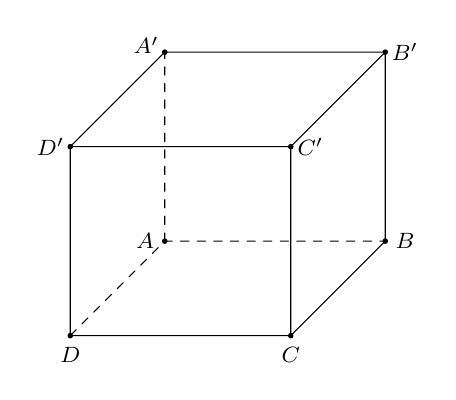
\begin{tikzpicture}[scale=0.8, font=\footnotesize, line join=round, line cap=round, >=stealth]
		\path
		(0,0) coordinate (D) 
		(3.5,0) coordinate (C) 
		(1.5,1.5) coordinate (A) 
		(A)+(3.5,0) coordinate (B);
		\foreach \x in {A,B,C,D}
		\path (\x)+(0,3) coordinate(\x');	
		\draw[dashed] (D)--(A)--(B) (A)--(A');
		\draw(D')--(C')--(B')--(A')--(D')--(D)--(C)--(B)--(B') (C)--(C');
		\foreach \p/\g in {D/-90,C/-90,B/0,A/180,D'/180,C'/0,B'/0,A'/160}\draw[fill=black] (\p) circle (1pt)node[shift={(\g:.25)}]{$\p$};
		\end{tikzpicture}}
	\loigiai{
		\immini{Ta có $\widehat{\left( AC,A'D \right)}=\widehat{\left( A'C',A'D \right)}=\widehat{DA'C'}=60^\circ $.
		Vì $A'D=A'C'=C'D$.}
		{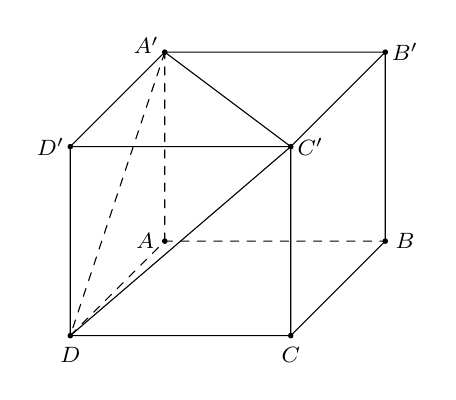
\begin{tikzpicture}[scale=0.8, font=\footnotesize, line join=round, line cap=round, >=stealth]
			\path
			(0,0) coordinate (D) 
			(3.5,0) coordinate (C) 
			(1.5,1.5) coordinate (A) 
			(A)+(3.5,0) coordinate (B);
			\foreach \x in {A,B,C,D}
			\path (\x)+(0,3) coordinate(\x');	
			\draw[dashed] (A')--(D)--(A)--(B) (A)--(A');
			\draw(D')--(C')--(B')--(A')--(D')--(D)--(C)--(B)--(B') (C')--(D) (C)--(C')--(A');
			\foreach \p/\g in {D/-90,C/-90,B/0,A/180,D'/180,C'/0,B'/0,A'/160}\draw[fill=black] (\p) circle (1pt)node[shift={(\g:.25)}]{$\p$};
		\end{tikzpicture}}
		}
\end{ex}

\begin{ex}%[1H8H2-2]
	Cho hình chóp $S.ABCD$ có đáy là hình bình hành tâm $O$, $SA=SC$, $SB=SD$. Trong các khẳng định sau khẳng định nào đúng?	
	\choice
		{$SA\perp (ABCD)$}
		{\True $SO\perp (ABCD)$}
		{$SC\perp (ABCD)$}
		{$SB\perp (ABCD)$}
	\loigiai{
		\immini{Ta có $O$ là trung điểm của $AC,BD$
		Mà $SA=SC,SB=SD\Rightarrow SO\perp AC,SO\perp BD$
		$\Rightarrow SO\perp (ABCD)$.}
		{\begin{tikzpicture}[>=stealth,line join=round,line cap=round,font=\footnotesize,scale=0.6]
				\path (0,0) coordinate (A)
				(6,0) coordinate (B)
				(-3,-2) coordinate (D)
				($(B)-(A)+(D)$) coordinate (C)
				($(A)!1/2!(C)$) coordinate (O)
				($(O)+(0,6)$) coordinate (S)
				; 
				\draw (C)--(S)--(D)--(C)--(B)--(S) 
				;
				\draw[dashed]
				(D)--(A)--(S)--(O)
				(C)--(A)--(B)--(D)
				;
				\foreach \p/\r in {A/150,B/0,C/-70,D/-90,O/-90,S/90}
				\fill (\p) circle (1pt) node[shift={(\r:3mm)}]{$\p$};
				\end{tikzpicture}}
		}
\end{ex}
  
\begin{ex}%[1H8B1-2]
	Cho hình chóp $S.ABC$ đáy $ABC$ là tam giác đều, cạnh bên $SA$ vuông góc với đáy. Gọi $M$, $N$ lần lượt là trung điểm của $AB$ và $SB$. Trong các mệnh đề sau, mệnh đề nào là mệnh đề đúng?
	\choice
		{$BC\perp SB$}
		{$BC\perp AN$}
		{$BC\perp MN$}
		{\True $BC\perp SM$}
	\loigiai{
		\immini{Ta có $\heva{
		  & BC\perp AM \\ 
		 & BC\perp SA \\ 
		 & SA,\,AM\subset (SAM)}\Rightarrow BC\perp (SAB)\Rightarrow BC\perp SM$.
		}
		 {\begin{tikzpicture}[font=\footnotesize, line join=round, line cap=round, >=stealth]
		 		\path 	(0,0) coordinate (A)
		 		(1.75,-1.75) coordinate (B)
		 		(4.5,0) coordinate (C)
		 		($(A)+(90:3)$) coordinate (S)
		 		($(B)!0.5!(C)$) coordinate (M)
		 		($(B)!0.5!(S)$) coordinate (N);
		 		\draw 	(C)--(B)--(A)--(N)
		 		(A)--(S)	(B)--(S)--(M)	(C)--(S)--(B);
		 		\draw[dashed] 	(M)--(A)--(C);
		 		\foreach \x /\goc in {A/180,B/-60,C/0,S/90,M/-30,N/0}
		 		\fill[black] (\x) circle (1pt)
		 		($(\x)+(\goc:3mm)$) node {$\x$};
		 \end{tikzpicture}}
		}
\end{ex}
  
\Closesolutionfile{ans}
\bangdapan{Dapan}

\subsection{Câu trắc nghiệm đúng sai}
Học sinh trả lời từ câu 1 đến câu 4.
Trong mỗi ý \circlenum{A}, \circlenum{B}, \circlenum{C} và \circlenum{D} ở mỗi câu, học sinh chọn đúng hoặc sai.
\setcounter{ex}{0}
\LGexTF
\Opensolutionfile{ansbook}[ansbook/DapanDS]
\Opensolutionfile{ans}[Ans/DapanT]
\begin{ex}%[1D6H2-1]
	Cho biểu thức $B=2\ln\sqrt{\mathrm{e}x}-\ln\dfrac{\mathrm{e}^2}{\sqrt{x}}+\ln 3\cdot\log_3\left(\mathrm{e}x^2\right)$. Vậy
	\choiceTF
	{\True Cho $\ln x=2$ thì $B=7$}
	{\True Cho $\ln x=4$ thì $B=14$}
	{Cho $\ln x=3$ thì $B=\dfrac{15}{2}$}
	{Cho $\ln x=6$ thì $B=18$}
	\loigiai{
		Ta có
		\begin{eqnarray*}
			B&=&2\ln(\mathrm{e}x)^{\tfrac{1}{2}}-\left(\ln\mathrm{e}^2-\ln x^{\tfrac{1}{2}}\right)+\ln\left(\mathrm{e}x^2\right)\\
			&=&\ln (\mathrm{e}x)-\left(2-\dfrac{1}{2}\ln x\right)+\ln\left(\mathrm{e}x^2\right)=(\ln \mathrm{e}+\ln x)-2+\dfrac{1}{2}\ln x+\ln \mathrm{e}+\ln x^2\\
			&=&1+\ln x-2+\dfrac{1}{2}\ln x+1+2\ln x=\dfrac{7}{2}\ln x.
		\end{eqnarray*}
		\begin{itemize}
			\item Với $\ln x=2$ suy ra $B=7$ vậy mệnh đề \lq\lq Cho $\ln x=2$ thì $B=7$\rq\rq\, đúng.
			\item Với $\ln x=4$ suy ra $B=14$ vậy mệnh đề \lq\lq Cho $\ln x=4$ thì $B=14$\rq\rq\, đúng.
			\item Với $\ln x=3$ suy ra $B=\dfrac{21}{2}$ vậy mệnh đề \lq\lq Cho $\ln x=2$ thì $B=\dfrac{15}{2}$\rq\rq\, sai.
			\item Với $\ln x=6$ suy ra $B=21$ vậy mệnh đề \lq\lq Cho $\ln x=6$ thì $B=18$\rq\rq\, sai.
		\end{itemize}
	}
\end{ex}
\begin{ex}%[1D6H4-5]
	Cho bất phương trình $\log_{0{,}5}(x+1)^2\leq\log_{0{,}5}2x$, có tập nghiệm là $S=(a;b)$. Khi đó:
	\choiceTF
	{\True $a=0$}
	{\True $(a;b)\cap(3;2024)=(3;2024)$}
	{$A(a;0)$ là tọa độ đỉnh của parabol $(P)\colon y=x^2+2$}
	{$\lim\limits_{x\to b}\left(\dfrac{1}{x^3}+\dfrac{1}{x^2}+\dfrac{1}{x}\right)=3$}
	\loigiai{
		Điều kiện: $\heva{&(x+1)^2>0\\&2x>0}\Leftrightarrow\heva{&x\neq-1\\&x>0}\Leftrightarrow x>0.\quad (*)$\\
		Khi đó, do cơ số $0<0{,}5<1$ nên bất phương trình đã cho trở thành
		$$(x+1)^2\geq 2x\Leftrightarrow (x-1)^2\geq 0\Leftrightarrow x\in\mathbb{R}.$$
		Kết hợp với điều kiện $(*)$, ta được tập nghiệm của bất phương trình là $S=(0;+\infty)$. Do đó $\heva{& a=0 \\ & b=+\infty.}$
		\begin{itemize}
			\item \lq\lq $a=0$\rq\rq\, đúng.
			\item Ta có $(a;b)\cap(3;2024)=(0;+\infty)\cap (3;2024)=(3;2024)$. Mệnh đề \lq\lq $(a;b)\cap(3;2024)=(3;2024)$\rq\rq\, đúng.
			\item Parabol $(P)\colon y=x^2+2$ có tọa độ đỉnh $A(0;2)$ nên mệnh đề \lq\lq $A(a;0)$ là tọa độ đỉnh của parabol $(P)\colon y=x^2+2$\rq\rq\, sai.
			\item Ta có $\lim\limits_{x\to b}\left(\dfrac{1}{x^3}+\dfrac{1}{x^2}+\dfrac{1}{x}\right)=\lim\limits_{x\to +\infty}\left(\dfrac{1}{x^3}+\dfrac{1}{x^2}+\dfrac{1}{x}\right)=0$ nên mệnh đề \lq\lq $\lim\limits_{x\to b}\left(\dfrac{1}{x^3}+\dfrac{1}{x^2}+\dfrac{1}{x}\right)=3$\rq\rq\, sai.
		\end{itemize}
	}
\end{ex}
\begin{ex}%[1H8H1-3]
	Cho tứ diện đều $ABCD$ có các cạnh bằng $a$. Gọi $M$, $N$ lần lượt là trung điểm của $AB$ và $CD$. Khi đó
	\choiceTF
	{$NA=NB=\dfrac{a\sqrt{3}}{3}$}
	{\True $MN=\dfrac{a\sqrt{2}}{2}$}
	{$\overrightarrow{MN}\cdot\overrightarrow{BC}=\dfrac{a^2}{3}$}
	{\True Góc giữa đường thẳng $MN$ và $BC$ bằng $45^{\circ}$}
	\loigiai{
		\begin{center}
			\begin{tikzpicture}[scale=1,font=\footnotesize,line join=round,line cap=round,>=stealth]
			\path
			(0,0) coordinate (B)
			(1,-2) coordinate (C)
			(4,0) coordinate (D)
			(1.2,3.4)coordinate (A)
			($(A)!0.5!(B)$) coordinate (M)
			($(C)!0.5!(D)$) coordinate (N)				
			;
			\draw (A)--(B)--(C)--(D)--cycle (N)--(A)--(C);
			\draw[dashed] (M)--(N)--(B)--(D);
			\foreach \p/\q in {A/90,B/180,C/-90,D/0,M/150,N/-30}
			\fill[black] (\p) circle (1.0pt) ($(\p)+(\q:2.5mm)$) node{$\p$};	
			\end{tikzpicture}
		\end{center}
		Ta có $AN$, $BN$ lần lượt là các đường trung tuyến của hai tam giác đều $\triangle ACD$ và $\triangle BCD$ nên $NA=NB=\dfrac{a\sqrt{3}}{2}$.\\
		Do đó $\triangle NAB$ cân tại $N$ và $MN\perp AB$.\\
		Xét $\triangle AMN$ vuông tại $M$. Ta có 
		$MN=\sqrt{AN^2-AM^2}=\sqrt{\left(\dfrac{a\sqrt{3}}{2}\right)^2-\left(\dfrac{a}{2}\right)^2}=\dfrac{a\sqrt{2}}{2}$.\\
		Đặt $\overrightarrow{AB}=\overrightarrow{a}$, $\overrightarrow{AC}=\overrightarrow{b}$, $\overrightarrow{AD}=\overrightarrow{c}$.\\
		$\overrightarrow{MN}=\overrightarrow{AN}-\overrightarrow{AM}=\dfrac{1}{2}\left(\overrightarrow{AC}+\overrightarrow{AD}\right)-\dfrac{1}{2}\overrightarrow{AB}=-\dfrac{1}{2}\overrightarrow{a}+\dfrac{1}{2}\overrightarrow{b}+\dfrac{1}{2}\overrightarrow{c}$.\\
		$\overrightarrow{BC}=\overrightarrow{AC}-\overrightarrow{AB}=-\overrightarrow{a}+\overrightarrow{b}$.\\
		$\overrightarrow{MN}\cdot\overrightarrow{BC}=(-\overrightarrow{a}+\overrightarrow{b})\left(-\dfrac{1}{2}\overrightarrow{a}+\dfrac{1}{2}\overrightarrow{b}+\dfrac{1}{2}\overrightarrow{c}\right)=\dfrac{1}{2}\left(\overrightarrow a^2-\overrightarrow{a}\cdot\overrightarrow{b}-\overrightarrow{a}\cdot\overrightarrow{c}-\overrightarrow{a}\cdot\overrightarrow{b}+\overrightarrow b^2+\overrightarrow{b}\cdot\overrightarrow{c}\right)$.\\
		Do $\overrightarrow{a}\cdot\overrightarrow{b}=\overrightarrow{a}\cdot\overrightarrow{c}=\overrightarrow{b}\cdot\overrightarrow{c}=a^2\cdot\cos 60^{\circ}=\dfrac{a^2}{2}$ và $\overrightarrow a^2=\overrightarrow b^2=\overrightarrow c^2$.\\
		Suy ra $\overrightarrow{MN}\cdot\overrightarrow{BC}=\dfrac{1}{2}\left(\overrightarrow a^2-\dfrac{1}{2}\overrightarrow a^2-\dfrac{1}{2}\overrightarrow a^2-\dfrac{1}{2}\overrightarrow a^2+\overrightarrow a^2+\dfrac{1}{2}\overrightarrow a^2\right)=\dfrac{a^2}{2}$.\\
		Gọi $\varphi$ là góc giữa $MN$ và $BC$.\\
		Ta có $\cos\varphi=\dfrac{\left|\overrightarrow{MN}\cdot\overrightarrow{BC}\right|}{\left|\overrightarrow{MN}\right|\cdot\left|\overrightarrow{BC}\right|}=\dfrac{\dfrac{a^2}{2}}{\dfrac{a\sqrt{2}}{2}\cdot a}=\dfrac{\sqrt{2}}{2}$.\\
		Suy ra $\varphi=45^{\circ}$ hay $(MN,BC)=45^{\circ}$.
		\begin{itemize}
			\item Vì $NA=NB=\dfrac{a\sqrt{3}}{2}$ nên mệnh đề \lq\lq $NA=NB=\dfrac{a\sqrt{3}}{3}$\rq\rq\, sai.
			\item Vì $MN=\dfrac{a\sqrt{2}}{2}$ nên mệnh đề \lq\lq $MN=\dfrac{a\sqrt{2}}{2}$\rq\rq\, đúng.
			\item Vì $\overrightarrow{MN}\cdot\overrightarrow{BC}=\dfrac{a^2}{2}$ nên mệnh đề \lq\lq $\overrightarrow{MN}\cdot\overrightarrow{BC}=\dfrac{a^2}{3}$\rq\rq\, sai.
			\item Vì $(MN,BC)=45^{\circ}$ nên mệnh đề \lq\lq Góc giữa đường thẳng $MN$ và $BC$ bằng $45^{\circ}$\rq\rq\, đúng.
		\end{itemize}
	}
\end{ex}
\begin{ex}%[1H8H2-2]
	Cho tam giác $ABC$ vuông tại $C$. Gọi $d$ là đường thẳng vuông góc với $(ABC)$ tại $A$, lấy điểm $S$ nằm trên $d$ không trùng với $A$. Hai điểm $E$ và $F$ lần lượt là hình chiếu của $A$ trên các cạnh $SC$ và $SB$. Khi đó:
	\choiceTF
	{\True $BC\perp (SAC)$}
	{\True $AE\perp BC$}
	{\True $AE\perp (SBC)$}
	{\True $SB\perp (AEF)$}
	\loigiai{
		\begin{center}
			\begin{tikzpicture}[scale=1, font=\footnotesize, line join=round, line cap=round,>=stealth]
			\path
			(0,0) coordinate (A)
			(1.5,-1.5) coordinate (C)
			(4,0) coordinate (B)
			($(A)+(0,3.3)$) coordinate (S)	
			($(S)!0.35!(C)$) coordinate (E)
			($(S)!0.45!(B)$) coordinate (F)
			;
			\draw (S)--(A)--(C)--(B)--cycle (S)--(C) (A)--(E)--(F);	
			\draw[dashed] (F)--(A)--(B);	
			\foreach \p/\q in {S/90,A/180,C/-90,B/0,E/60,F/50}
			\fill[black] (\p) circle (1.0pt) ($(\p)+(\q:2.5mm)$) node{$\p$};
			\draw pic[draw=black,angle radius=0.2cm] {right angle = B--C--A}
			pic[draw=black,angle radius=0.2cm] {right angle = A--E--C}
			pic[draw=black,angle radius=0.2cm] {right angle = A--F--B}; 
			\end{tikzpicture}
		\end{center}
		Ta có $\heva{&BC\perp AC\\&BC\perp SA}\Rightarrow BC\perp (SAC)$.\\
		Ta có $BC\perp (SAC)$.\\
		Mà $AE\subset (SAC)\Rightarrow BC\perp AE$.\\
		Ta có $SB\perp AF.\quad (1)$\\
		$\heva{&AE\perp SC\\&AE\perp BC\text{ (do } BC\perp (SAC))}\Rightarrow AE\perp (SBC).\quad(2)$\\
		Từ $(1)$ và $(2)$ suy ra $SB\perp (AEF)$.
		\begin{itemize}
			\item Mệnh đề \lq\lq $BC\perp (SAC)$\rq\rq\, đúng.
			\item Mệnh đề \lq\lq $AE\perp BC$\rq\rq\, đúng.
			\item Mệnh đề \lq\lq $AE\perp (SBC)$\rq\rq\, đúng.
			\item Mệnh đề \lq\lq $SB\perp (AEF)$\rq\rq\, đúng.
		\end{itemize}
	}
\end{ex}

\Closesolutionfile{ans}
\Closesolutionfile{ansbook}

\begin{center}
	\textbf{\textsf{BẢNG ĐÁP ÁN ĐÚNG SAI}}
\end{center}
\input{Ansbook/DapanDS}

\subsection{Phần tự luận}

\hienthiloigiaibt
%%%=============BT_1=============%%%
\begin{bt}%[1D6V2-1]
Biết $4^x+4^{-x}=23$, tính giá trị của biểu thức $P=2^x+2^{-x}$.
\loigiai{
	\begin{enumerate}[$\bullet$]
		\item Ta có $4^x+4^{-x}=23 \Leftrightarrow (2^x+2^{-x})^2=25 \Leftrightarrow \hoac{&2^x+2^{-x}=5\\ &2^x+2^{-x}=-5}$.
		\item Do $2^x+2^{-x}>0$ nên $2^x+2^{-x}=5$.
	\end{enumerate}
	}
\end{bt}
\begin{bt}%[1D6V4-2]
Trong nông nghiệp bèo hoa dâu được dùng làm phân bón, nó rất tốt cho cây trồng. Mới đây, các nhà khoa học Việt Nam đã phát hiện ra bèo hoa dâu có thể dùng để chiết xuất ra chất có tác dụng kích thích hệ miễn dịch và hỗ trợ điều trị bệnh ung thư. Bèo hoa dâu được thả nuôi trên mặt nước. Một người đã thả một lượng bèo hoa dâu chiếm $4 \%$ diện tích mặt hồ. Biết rằng cứ sau đúng một tuần bèo phát triển thành 3 lần số lượng đã có và giả sử tốc độ phát triển của bèo ở mọi thời điểm như nhau. Hỏi sau ít nhất bao nhiêu ngày bèo sẽ vừa phủ kín mặt hồ?
	\loigiai{
		\begin{enumerate}[$\bullet$]
			\item Số lượng bèo ban đầu chiếm $0{,}04$ diện tích mặt hồ.
			\item Sau 1 tuần số lượng bèo là $0{,}04 \times 3$ diện tích mặt hồ.
			\item Sau 2 tuần số lượng bèo là $0{,}04 \times 3^2$ diện tích mặt hồ.
			\item Sau $n$ tuần số lượng bèo là $0{,}04 \times 3^n$ diện tích mặt hồ.
			\item 	Để bèo phủ kín mặt hồ thì: $0{,}04 \times 3^n=1 \Rightarrow 3^n=25 \Rightarrow n=\log _3 25$ (tuần).
			\item Số ngày tương ứng là $7 n=7 \log _3 25 \approx 20,51$ (ngày).
		\end{enumerate}
		Vậy sau ít nhất 21 ngày thì bèo hoa dâu sẽ phủ kín mặt hồ.
	}
\end{bt}
\begin{bt}%[1D6V2-4]
Ông Quý dự định gửi vào ngân hàng một số tiền với lãi suất $6{,}5 \%$ một năm. Biết rằng, cứ sau mỗi năm số tiền lãi sẽ được nhập vào vốn ban đầu. Tính số tiền tối thiểu $x$ (triệu đồng, $x \in \mathbb{N}$) ông Quý gửi vào ngân hàng để sau 3 năm số tiền lãi đủ mua một chiếc xe gắn máy trị giá 30 triệu đồng.
	\loigiai{
		\begin{enumerate}[$\bullet$]
		\item 	Công thức lãi kép $T=A(1+r)^n$.
		\item Tiền lãi ông Quý có sau 3 năm sẽ là tiền gốc lẫn lãi trừ đi số tiền gốc ban đầu. Ta có: $A(1+6,5 \%)^3-A \geq 30 \Leftrightarrow A \geq \dfrac{30}{(1+6,5 \%)^3-1} \approx 144{,}26$ triệu.
		\item Do $x \in \mathbf{N}$ nên $x=145$ triệu đồng.
	\end{enumerate}
	}
\end{bt}
\begin{bt}%[1D6V4-2]
Giải phương trình $\log _2[x(x-1)]=1$.
	\loigiai{
		\begin{enumerate}[$\bullet$]
			\item 	Ta có $\log _2[x(x-1)]=1 \Leftrightarrow x(x-1)=2 \Leftrightarrow x^2-x-2=0 \Leftrightarrow \hoac{& x=-1\\ &x=2}$.
		\end{enumerate}
Vậy phương trình có nghiệm là $x=-1; x=2$.
	}
\end{bt}
\begin{bt}%[1H8V1-3]
	Cho hình chóp $S.ABC$ có $AB=AC, \,\widehat{SAC}=\widehat{SAB}$. Tính số đo của góc giữa hai đường thẳng $SA$ và $BC$.
	\loigiai{
		\immini{\begin{enumerate}[$\bullet$]
				\item  Ta có $\vec{SA}\cdot\vec{BC}=\vec{SA}\cdot(\vec{SB}-\vec{SC})\\=SA\cdot SB\cdot\cos\widehat{SAB}-SA\cdot SC\cdot \cos\widehat{SAC}=0$.
				\item $(SA{,}BC)=90^{\circ}$.
		\end{enumerate}}
		{
				\begin{tikzpicture}[scale=0.7,font=\footnotesize,line join=round,line cap=round,>=stealth]
				\path
				(0,2) coordinate (A)
				(5,2) coordinate (B)
				(3.5,0.5) coordinate (C)
				(2.5,6)coordinate (S)
				($(B)!0.5!(C)$) coordinate (M);
				\draw (A)--(C)--(S)--(B)--(C) (S)--(A) (S)--(M);
				\draw[dashed] (A)--(B) (A)--(M);
				\foreach \p/\q in {A/180,B/0,C/-90,S/90,M/0}
				\fill[black] (\p) circle (1.0pt) ($(\p)+(\q:2.5mm)$) node{$\p$};	
				\end{tikzpicture}
	}	}
\end{bt}
\begin{bt}%[1H8V1-3]
Cho tứ diện $ABCD$ có $AC=AD, BC=BD$. Tìm số đo của góc $(CD{,} AB)$.
	\loigiai{
	\immini{\begin{enumerate}[$\bullet$]
			\item  Gọi $I$ là trung điểm của $CD$.
			\item  Ta có:
			$$
			\left\{\begin{array}{l}
			C D \perp B I \\
			C D \perp A I
			\end{array} \Rightarrow C D \perp(A B I) \Rightarrow C D \perp A B\right.
			$$
				\item $(AB,CD)=90^{\circ}$.
	\end{enumerate}}
	{
		\begin{tikzpicture}[scale=0.7,font=\footnotesize,line join=round,line cap=round,>=stealth]
		\path
		(0,2) coordinate (B)
		(5,2) coordinate (D)
		(3.5,0.5) coordinate (C)
		(2.5,6)coordinate (A)
		($(C)!0.5!(D)$) coordinate (I);
		\draw (A)--(B)--(C)--(D)--(A) (A)--(C) (A)--(I);
		\draw[dashed] (B)--(D) (B)--(I);
		\foreach \p/\q in {B/180,D/0,C/-90,A/90,I/0}
		\fill[black] (\p) circle (1.0pt) ($(\p)+(\q:2.5mm)$) node{$\p$};	
		\end{tikzpicture}
}	}
\end{bt}
